\documentclass{beamer}
\usepackage[spanish]{babel}
\usepackage[utf8]{inputenc}
\usepackage{graphicx}


\newtheorem{procedimiento}{¿En que nos hemos centrado?}
\newtheorem{forma}{¿Como miramos la eficiencia de la interpolación de Taylor?}
\newtheorem{idea}{¿En que consiste la interpolación de Taylor?}
\newtheorem{descripcion de los experimentos}{\underline {Descripcion de los experimentos}}
\newtheorem{introduccion}{\underline {Introducci\'{o}n}}
\newtheorem{objetivos}{\underline {Objetivos}}
\newtheorem{material}{\underline {Material utilizado}}
\newtheorem{resultados}{\underline {Resultados}}
\newtheorem{analisis}{\underline {Analisis de los resultados}}
\newtheorem{ademas}{\underline {ademas}}
\newtheorem{hola}{Segunda tabla}
\newtheorem{adios}{Tercera tabla}


\title[Presentación con Beamer]{Trabajo final: Interpolación de Taylor.}
\author[Técnicas Experimentales]{Bolaños Florido,Cynthia. \\
Cruz Guerra, Adrián.\\
Díaz Rodríguez, Diego}
\date[15-05-2013]{Miércoles 15 de marzo de 2013}


\usetheme{classic}

\begin{document}


\begin{frame}


\includegraphics[width=0.15\textwidth]{img/ullesc.eps}
\hspace*{7.5cm}

\includegraphics[width=0.16\textwidth]{img/fmatesc.eps}
\titlepage

  \begin{scriptsize}
    \begin{center}
     Facultad de Matemáticas \\
     Universidad de La Laguna \\
     Grupo 1I.
    \end{center}
  \end{scriptsize}
\end{frame}


\begin{frame}
  \frametitle{Índice}
  \tableofcontents[pausesections]
\end{frame}


\section{Objetivos.}
\begin{frame}
\frametitle{Objetivos.}
\begin{introduccion}
El siguiente informe científico-técnico ha sido realizado para exponer, explicar y analizar la interpolación de Taylor de una función.
\pause
\end{introduccion}
\begin{objetivos}
\pause
\begin {itemize}
\item \underline {Objetivo principal:} Interpolación  de Taylor de la  función:
\textcolor{blue}{$$f(x)= \frac{1}{4x}$$}
\item \underline {Objetivo secundario:} Familiarizarnos con LaTeX
\end {itemize}
\end{objetivos}
\end{frame}


\section{Procedimiento experimental.}
\begin{frame}
\frametitle{Procedimiento experimental.}
\begin {descripcion de los experimentos}
\begin{idea}
\pause
\begin {itemize}
\item Aplicar la suseción de Taylor:
\textcolor{blue}{$$P_n(f,x,c)=f(c)+\frac{f'(c)}{1!}(x-c)+\frac{f''(c)}{2!}(x-c)^2+ \cdots +\frac{f^{n)}(c)}{n!}(x-c)^n$$}
\end {itemize}
\pause
\end {idea}
\begin{procedimiento}
\begin {itemize}
\item Grado de Taylor
\item Relación de $x$ y $c$ con Taylor.
\end {itemize}
\end {procedimiento}
\end{descripcion de los experimentos}
\end{frame}


\begin{frame}
\begin{forma}
\pause
\begin {itemize}
\item Comparar la función con la interpolada:
\textcolor{blue}{$$P_n(f,x,c)=f(c)+\frac{f'(c)}{1!}(x-c)+\frac{f''(c)}{2!}(x-c)^2+ \cdots +\frac{f^{n)}(c)}{n!}(x-c)^n$$
$$f(x)= \frac{1}{4x}$$}
\end {itemize}
\end {forma}
\end {frame}


\begin {frame}
\begin{material}
\pause
El material utilizado ha sido el siguiente:
\begin {itemize}
\item \underline{Tipo de CPU}: 

\begin {center}
 Pentium(R) Dual-Core CPU E5200 @ 2.50GHz 
\end {center}
\item \underline{Tamaño de la memoria del procesador}: 

\begin {center}
 2048 KB
\end {center}
\item \underline{Vendedor GenuineIntel}:

\begin {center}
Linux
\end {center}
\end {itemize}
\end {material}
\end {frame}
\begin{frame}
\begin {itemize}
\item \underline{Sistema operativo}:

\begin {center}
 66-Ubuntu SMP
\end {center}
\item \underline{Plataforma}:

\begin {center}
 Linuz-3.2.0-41-generic-i686-with-Ubuntu-12.04-precise
\end {center}
\item \underline{Version}:

\begin {center}
2.7.3
\end {center}
\end {itemize}
\end{frame}


\section{Conclusiones.}
\begin{frame}
\frametitle{Conclusiones.}
\begin{resultados}
Los resultados obtenidos se recogen en la siguiente tabla:
\begin{table}[!hbt]
\begin{center}\label{transparencia tabla 1}
\begin{tabular}[c]{||l | l ||l|l||}
\hline
\hline
$x$ & $f(x)=\frac{1}{4x}$ &{\em Taylor} & Error \\
\hline
1 &0.25& 0.01875 & 25\\
\hline
1.5 &0.1666667&0.15625& 6.25\\
\hline
2 &0.125 &0.125 & 0 \\
\hline
2.5 &0.1 &0.09375 & 6.25 \\
\hline
3 & 0.08333 & 0.0625 & 25 \\
\hline
\hline
\end{tabular}
\caption{La $c$ vale 2 y está interpolada en grado 1}
\end{center}
\end{table}
\hfill \hyperlink{transparencia grafica1}{\beamergotobutton{transparencia grafica1}}
\end{resultados}
\end{frame}


\begin{frame}
\begin{table}[!hbt]\label{transparencia tabla 2}
\begin{center}
\begin{tabular}[c]{||l | l ||l|l||}
\hline
\hline
$x$ & $f(x)=\frac{1}{4x}$ &{\em Taylor} & Error \\
\hline
1 &0.25 & 0.21875 &12.5 \\
\hline
1.5 &0.1666667 & 0.1640625& 1.5625 \\
\hline
2 &0.125 &0.125 & 0 \\
\hline
2.5 &0.1 &0.1015625 & 1.5625 \\
\hline
3 & 0.08333 & 0.09375& 12.5 \\
\hline
\hline
\end{tabular}
\caption{La $c$ vale 2 y está interpolada en grado 2}
\end{center}
\end{table}
\hfill \hyperlink{transparencia grafica2}{\beamergotobutton{transparencia grafica2}}
\end{frame}

\begin{frame}
\begin{table}[!hbt]\label{transparencia tabla 3}
\begin{center}
\begin{tabular}[c]{||l | l ||l|l||}
\hline
\hline
$x$ & $f(x)=\frac{1}{4x}$ &{\em Taylor} & Error \\
\hline
1 &0.25& 0.234375 & 6.25 \\
\hline
1.5 &0.1666667&0.166015625& 0.390625\\
\hline
2 &0.125 &0.125 & 0 \\
\hline
2.5 &0.1 &0.099609375 & 0.390625 \\
\hline
3 & 0.0.078125 & 0.234275& 6.25 \\
\hline
\hline
\end{tabular}
\caption{La $c$ vale 2 y está interpolada en grado 3}
\end{center}
\end{table}
\hfill \hyperlink{transparencia grafica3}{\beamergotobutton{transparencia grafica3}}
\end{frame}


\begin{frame}
\hfill \hyperlink{transparencia tabla 1}{\beamergotobutton{transparencia tabla 1}}
\begin{figure}\label{transparencia grafica1}
  \caption{Comportamiento gráfico de la función $f(x)=\frac{1}{4x}$ interpolada con Taylor con $c=2$ y de orden 1}
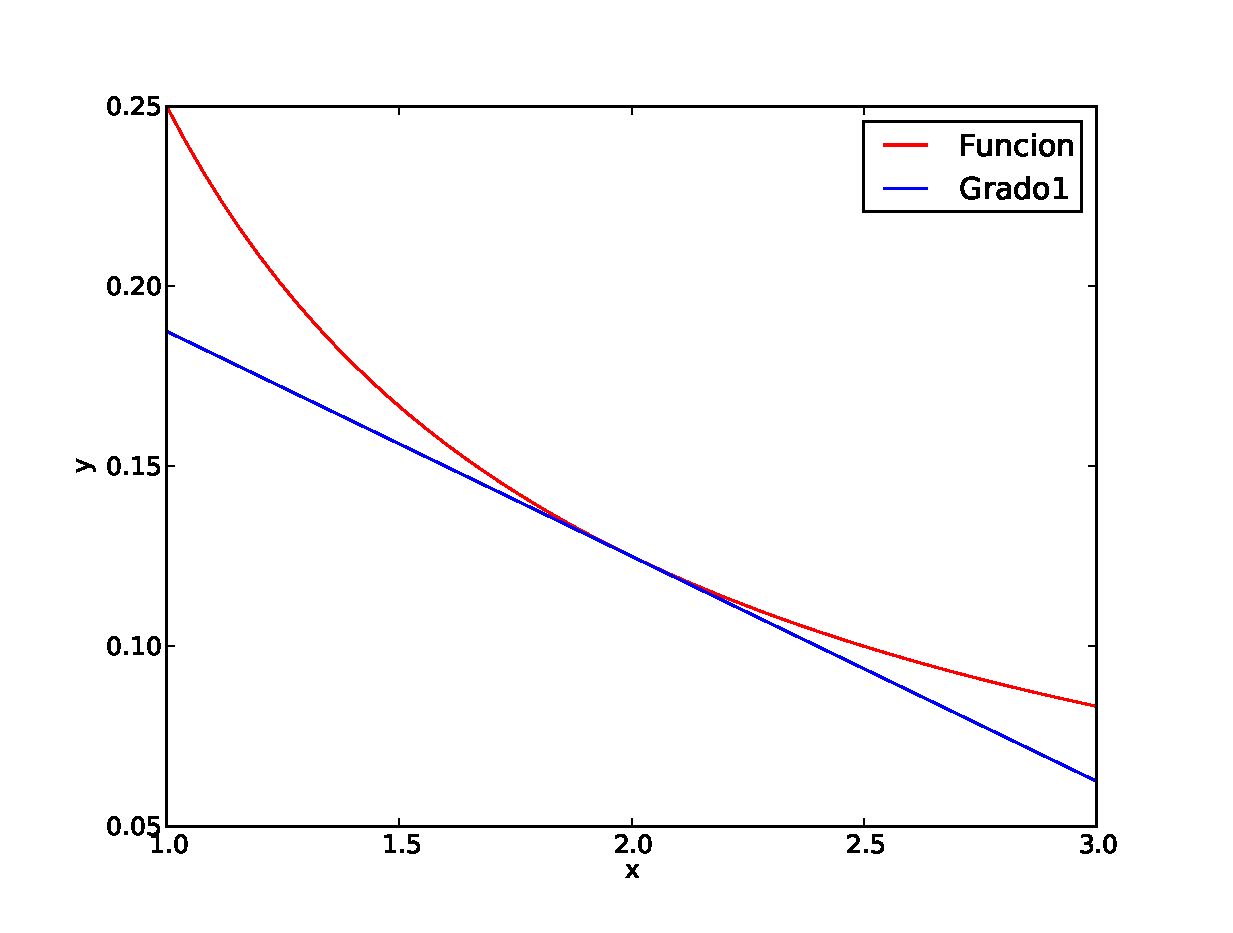
\includegraphics[width=10cm]{img/segunda.eps}
\end{figure}
\end{frame}


\begin{frame}
\hfill \hyperlink{transparencia tabla 2}{\beamergotobutton{transparencia tabla 2}}
\begin{figure}\label{transparencia grafica2}
  \caption{Comportamiento gráfico de la función $f(x)=\frac{1}{4x}$ interpolada con Taylor con $c=2$ y de orden 2}
  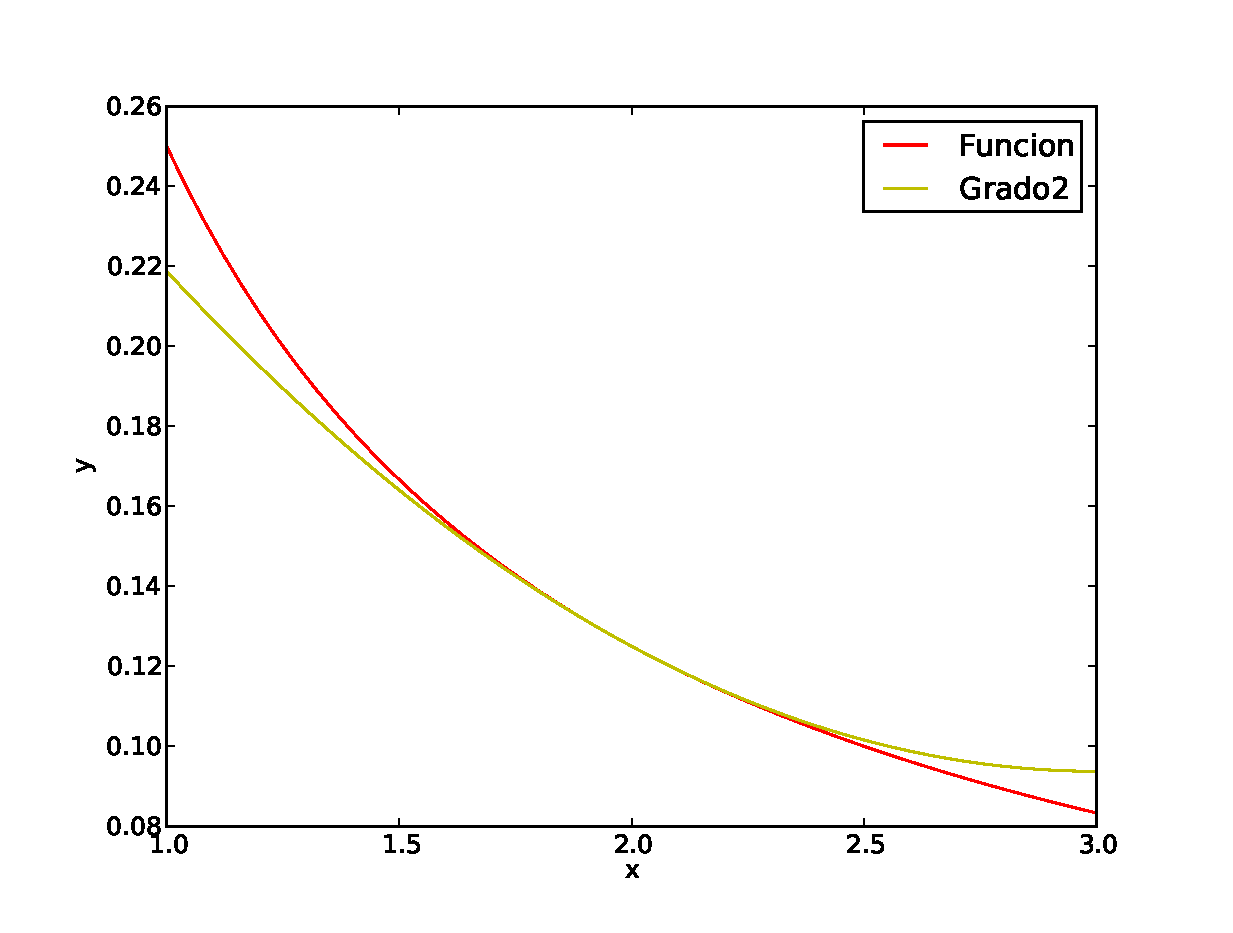
\includegraphics[width=10cm]{img/tercera.eps}
\end{figure}
\end{frame}


\begin{frame}
\hfill \hyperlink{transparencia tabla 3}{\beamergotobutton{transparencia tabla 3}}
\hfill \hyperlink{siguiente}{\beamergotobutton{siguiente}}
\begin{figure}\label{transparencia grafica3}
  \caption{Comportamiento gráfico de la función $f(x)=\frac{1}{4x}$ interpolada con Taylor con $c=2$ y de orden 3}
  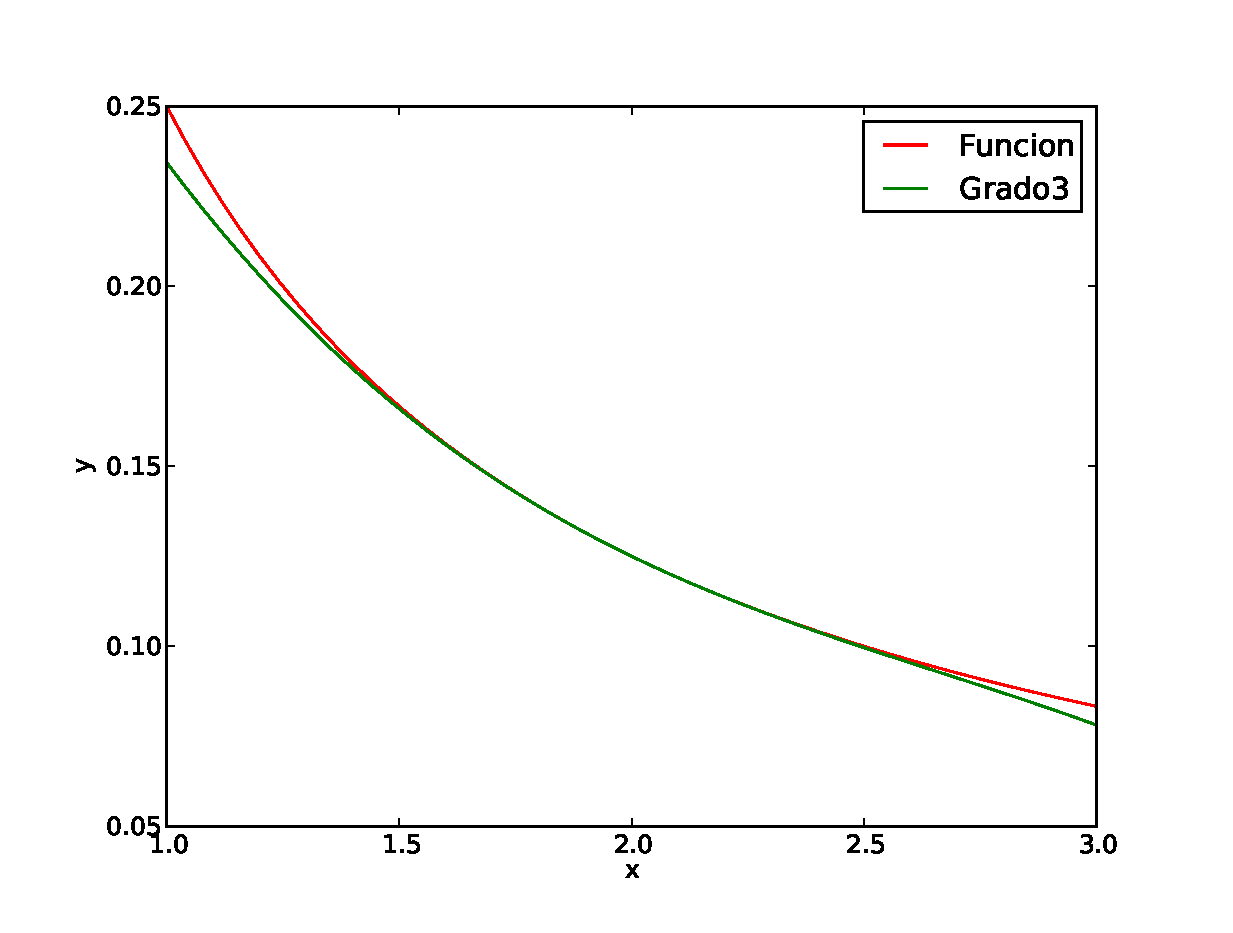
\includegraphics[width=10cm]{img/cuarta.eps}
\end{figure}
\end{frame}

\begin{frame}\label{siguiente}
\begin{figure}
  \caption{Comportamiento gráfico de la función $f(x)=\frac{1}{4x}$ con la interpolada en $c=2$ de orden 1,2,3}
  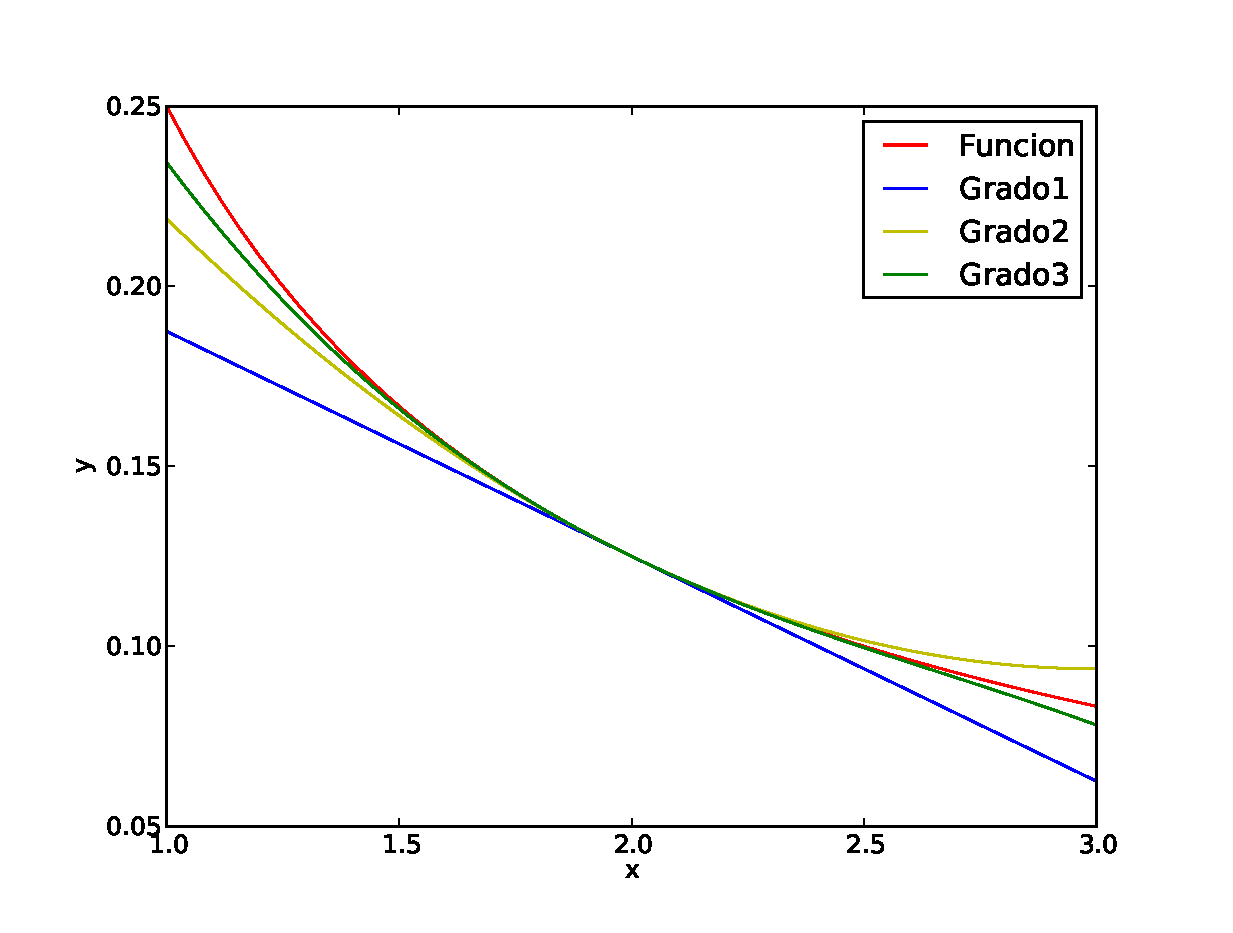
\includegraphics[width=10cm]{img/sexta.eps}
\end{figure}
\end{frame}

\begin{frame}
\begin{analisis}
En líneas generales se concluye que el error es menor:
\begin {itemize}
\item Cuanto mayor sea el grado de la derivada en la sucesión de Taylor.
\item Cuanto más próximo sea el valor de x respecto de c.
\end {itemize}
\begin {block}{Si c y x poseen el mismo valor entonces el error es 0.}
\end{block}
\end{analisis}
\end{frame}


\section{Bibliografia}
\begin{frame}
 \frametitle{Bibliografía}

   La información requerida para la realización de este informe ha sido extraída de las siguientes fuentes:

  \begin{thebibliography}{10}
    \beamertemplatebookbibitems
    \bibitem[Bibliografía]{listado}
\begin{itemize}
\item \href{disi.unal.edu.co/~lctorres/MetNum/MeNuI03.pdf}{$disi.unal.edu.co/~lctorres/MetNum/MeNuI03.pdf$}
\item \href{www.ugr.es/~mpasadas/ftp/Inter2.pdf}{$www.ugr.es/~mpasadas/ftp/Inter2.pdf$}
\item \href{cse.web.cs.illinois.edu/iem/interpolation/taylor/}{$cse.web.cs.illinois.edu/iem/interpolation/taylor/$}
\end {itemize}
  \end{thebibliography}
\end{frame}


\end{document}









